\documentclass{standalone}

\usepackage{circuitikz}

\begin{document}

% INT_AY21_L32_Fig03_Intersecting_lines.png

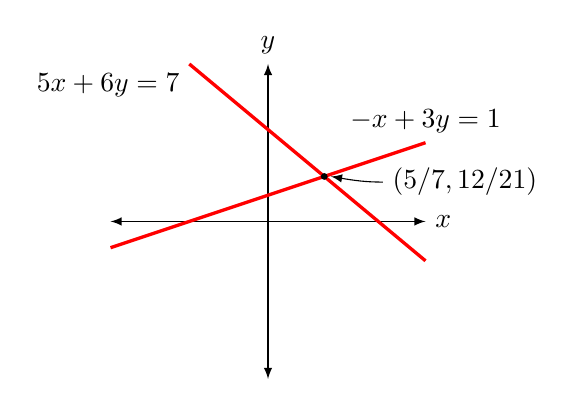
\begin{tikzpicture}[> = latex]

	% Axes
	
	\draw [<->] (-2, 0) -- (2, 0) node [right] {$x$};
	\draw [<->] (0, -2) -- (0, 2) node [above] {$y$};
	
	% Lines w/equations
	
	\begin{scope}[red, very thick]
	
		\draw (-1, 2) -- (2, -1/2);
		\draw (-2, -1/3) -- (2, 1);
		
	\end{scope}
	
	\node [below left] at (-1, 2) {$5x + 6y = 7$};
	\node [above] at (2, 1) {$-x + 3y = 1$};
	
	% Intersection point
	
	\filldraw (5/7, 12/21) circle (1 pt);
	\node (coords) at (2.5, 0.5) {$(5/7, 12/21)$};
	\draw [->] (coords.west) to [out = 180, in = -10] (0.8, 12/21);

\end{tikzpicture}

\end{document}